\chapter{量子网络望远镜}
\label{chap:e24}

\begin{chapteropening}
第 \ref{chap:e09} 章我们学会了把两台望远镜的光合到一起、数条纹：条纹的可见度就是复可见度 \(V\)，而 \(V\) 藏着恒星的角结构。可那一章也留下一个沉重的脚注——要让条纹稳定，两条光路的光程差必须锁在远小于一个波长的精度上，而且任何一路上的损耗都会\emph{直接吞掉本就稀少的星光光子}。基线拉到几公里、几十公里，这两条要求就双双失控。本章要问一个大胆的问题：能不能\emph{不把未知的星光长途搬运}，却仍然把两台相隔很远的望远镜"接成一台"？答案来自量子信息：预先制备好、可以验证、失败还能重来的\textbf{纠缠资源}（entanglement resource），加上\textbf{量子存储}（quantum memory）与\textbf{量子中继}（quantum repeater），让两端"共享"一个单光子的相位关系，而不必让那个脆弱的星光光子亲自跑完全程。这条路线目前还不是一台成熟的仪器，而是一张需要一项项算清的可行性账本；本章就带你把这张账本从头搭起来，并和第 \ref{chap:e10} 章的强度干涉摆在一起对照。
\end{chapteropening}

\section{为什么长基线的振幅干涉被光子损耗掐住}
\label{sec:e24-why-loss}

先把问题剥到最小。我们真正想保住的，不是"更多的光"，而是\emph{一阶相干的那个相位}。设想天空里一个点源，在一个相干时间 \(\tau_c\simeq1/\Delta\nu\)（第 \ref{chap:e02} 章）的时间窗里，恰好有一个来自它的光子飞到望远镜阵。极弱星光的关键事实是：每个时间窗里来自天体的平均光子数 \(\epsilon\ll1\)，绝大多数窗口是空的，偶尔一个窗口里只有一个光子。这一个光子，如果在到达探测器之前没有被"它究竟走了哪条路"这种信息污染，它就\emph{不是}"已经属于左望远镜"或"已经属于右望远镜"的经典粒子，而是左、右两条接收路径的量子叠加：

\begin{equation}
  |\psi_\star\rangle
  =
  \frac{|1\rangle_L|0\rangle_R
  +
  e^{i\phi}\,|0\rangle_L|1\rangle_R}{\sqrt2},
  \qquad
  \phi=\frac{2\pi\,\bm{B}\cdot\bm{\theta}}{\lambda}.
  \label{eq:e24-stellar-single-photon}
\end{equation}
\begin{formulaexplain}
\(|\psi_\star\rangle\) 是一个星光光子在左右两孔径之间的路径叠加态；\(|1\rangle_L|0\rangle_R\) 表示"左边有一个光子、右边为空"，另一项相反。\(\phi\) 是由基线 \(\bm{B}\)、源角位置 \(\bm{\theta}\) 与波长 \(\lambda\) 定出的几何相位。振幅干涉要保住的正是这个 \(\phi\)。
\end{formulaexplain}

这里 \(|1\rangle_L|0\rangle_R\) 是数态记号（第 \ref{chap:e05} 章）：下标 \(L,R\) 标记左、右两个空间模式，括号里的数字是该模式的光子数。\(\bm{B}\) 是投影基线（单位 cm，量级从 \(10^2\,\mathrm{cm}\) 到 \(10^7\,\mathrm{cm}\)），\(\bm{\theta}\) 是点源相对相位中心的角位置（无量纲弧度），\(\lambda\) 是波长（可见光 \(\sim6\times10^{-5}\,\mathrm{cm}\)）。相位 \(\phi\) 无量纲，是纯几何量——它就是第 \ref{chap:e09} 章条纹里的那个相位，只不过现在写成了单光子叠加态的语言。

真实恒星不是点，而是许多互不相干的点源之和（这正是第 \ref{chap:e10} 章 van Cittert--Zernike 定理的出发点）。每个子源 \(j\) 各自给出一个相位 \(\phi_j\) 的纯态 \eqref{eq:e24-stellar-single-photon}，非相干叠加就是把这些纯态按亮度加权求和成一个混合态；求和后，非对角元里出现的正是那些相位因子的加权平均 \(\langle e^{i(\phi_j-\phi_k)}\rangle\)，它恰好收敛成第 \ref{chap:e10} 章那个复可见度 \(V\)。只看单光子子空间 \(\{|10\rangle,|01\rangle\}\)，它的密度矩阵是

\begin{equation}
  \rho_1
  =
  \frac{1}{2}
  \begin{pmatrix}
  1 & V\\[2pt]
  V^* & 1
  \end{pmatrix}_{\{|10\rangle,\,|01\rangle\}} ,
  \qquad
  V=|V|\,e^{i\arg V}.
  \label{eq:e24-single-photon-density}
\end{equation}
\begin{formulaexplain}
\(\rho_1\) 是单光子子空间的密度矩阵；对角元 \(\tfrac12\) 只说明"光子可在任一台望远镜出现"，非对角元 \(V\) 才是复可见度，装着源的相干相位和角结构。\(|V|\) 从 1（点源）降到 0（源大到解析开），相位则给出源的位置与不对称。
\end{formulaexplain}

请对照第 \ref{chap:e10} 章式 \eqref{eq:e10-gamma12}：那里的复可见度 \(\gamma^{(1)}_{12}\) 是用两路场的时间平均定义的，这里的 \(V\) 就是同一个量，只是搬进了单光子密度矩阵的非对角元。物理含义完全一致：\emph{把 \(V\) 测出来，就等于测到了恒星}。传统振幅干涉的做法，是把 \(L,R\) 两个空间模式用光纤或自由空间光路送到\emph{同一个}合束器（beamsplitter）上，让 \(\phi\) 变成可数的条纹。麻烦就出在"送到同一个合束器"这一步：其中一路若走过长度 \(L\) 的有损链路，单光子透过率是

\begin{equation}
  \eta_{\rm ch}(L)=10^{-\alpha_{\rm dB}L/10}.
  \label{eq:e24-link-loss}
\end{equation}
\begin{formulaexplain}
\(\eta_{\rm ch}\) 是链路透过率（无量纲，\(0\) 到 \(1\)）；\(\alpha_{\rm dB}\) 是每公里的分贝损耗（单位 \(\mathrm{dB\,km^{-1}}\)），\(L\) 是链路长度（km）。分贝损耗让透过率随距离\emph{指数}衰减——这就是长基线直接光学合束的核心瓶颈。
\end{formulaexplain}

分贝是个对数刻度：\(10\,\mathrm{dB}\) 表示衰减到 \(1/10\)，\(20\,\mathrm{dB}\) 表示 \(1/100\)。把真实数字代进去感受一下。可见光在普通光纤里的损耗高达 \(20\)–\(30\,\mathrm{dB\,km^{-1}}\)，走 \(1\,\mathrm{km}\) 就只剩 \(10^{-2}\) 到 \(10^{-3}\) 以下——本就 \(\epsilon\ll1\) 的星光，几乎被吃干净。换到 \(1550\,\mathrm{nm}\) 的电信波段（telecom band），最好的光纤能低到 \(\sim0.2\,\mathrm{dB\,km^{-1}}\)，可星光并不天生长在这个波段，要先做频率转换、耦合、相位稳定，每一步都再乘一个小于 1 的效率；晴空自由空间链路可用 \(\sim0.5\,\mathrm{dB\,km^{-1}}\) 做量级估算，但大气湍流和指向误差带来的损失并不是这条干净的指数律 \citep{2012PhRvL.109g0503G,2019PhRvL.123g0504K,2024SPIE13095E..1NR}。一句话：\emph{你越想拉长基线，就越要把这个本来就稀缺的星光光子送得更远，而它被丢掉的概率随距离指数上升}。

\begin{figure}[tbp]
\centering
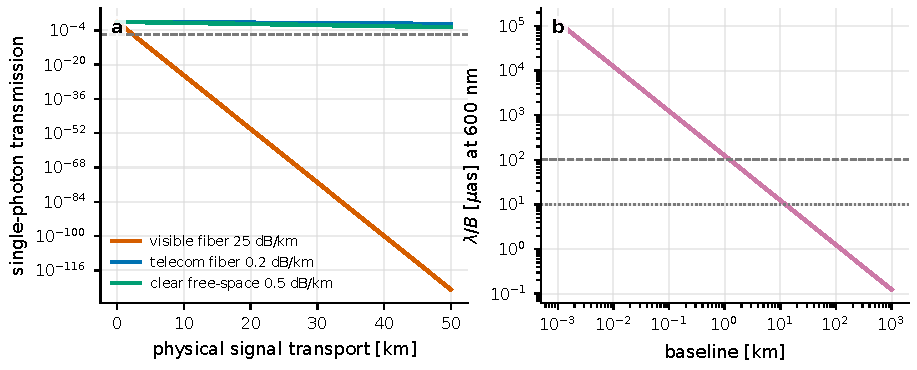
\includegraphics[width=0.94\linewidth]{figures/generated/chapter_17/ch17_architecture_loss.pdf}
\caption{长基线的诱惑与困难来自同一个量纲。左图把"直接传输单光子星光"的几种链路损耗画成透过率：可见光光纤在公里尺度就已严重衰减，电信波段光纤也会在百公里尺度变得昂贵。右图给出角分辨率标度 \(\lambda/B\)：\(600\,\mathrm{nm}\) 的光在 \(1\,\mathrm{km}\) 基线上达到百微角秒量级，\(100\,\mathrm{km}\) 基线进入微角秒量级。}
\label{fig:e24-architecture-loss}
\end{figure}

那为什么还要费这么大劲拉长基线？因为角分辨率的基本标度只认基线长度 \(B\)：

\begin{equation}
  \theta_{\rm res}\sim\frac{\lambda}{B}
  =124\,\mu\mathrm{as}
  \left(\frac{\lambda}{600\,\mathrm{nm}}\right)
  \left(\frac{1\,\mathrm{km}}{B}\right).
  \label{eq:e24-resolution-scale}
\end{equation}
\begin{formulaexplain}
\(\theta_{\rm res}\) 是干涉的角分辨率标度（这里用微角秒 \(\mu\mathrm{as}\)），\(B\) 是基线长度。基线越长，能分辨的角结构越细。量子网络方案追求的，正是在\emph{不长途搬运未知星光}的前提下，把 \(B\) 推到公里乃至更远。
\end{formulaexplain}

把括号里的比值代成 1，就读出 \(124\,\mu\mathrm{as}\) 这个基准；\(B=10\,\mathrm{km}\) 给 \(12\,\mu\mathrm{as}\)，\(B=100\,\mathrm{km}\) 给 \(1.2\,\mu\mathrm{as}\)。作为参照，最大的光学干涉阵列（如 CHARA）基线约几百米，只能到毫角秒级。量子网络望远镜的吸引力就锁在这个尺度上：它未必提高单孔径的灵敏度，却可能把光学/近红外干涉从几百米一路推向公里、十公里甚至更长。第 \ref{chap:e10} 章的强度干涉（HBT）其实早就绕开了光程传输这道坎——它不合束、只在本地记录强度涨落再离线相关，因此几乎不怕大气抖动，代价是它主要给 \(|V|^2\)，把相位丢了。量子网络路线的野心不同：它想\emph{保住一阶相干的相位}，同时又\emph{不把未知星光搬运长途}。

\section{预共享纠缠：把要长途搬运的东西换掉}
\label{sec:e24-gjc}

核心的一招，Gottesman--Jennewein--Croke 想出来了：既然长途搬运脆弱的未知星光如此昂贵，那就\emph{别搬它}，改搬一个我们完全掌握、可以验证、坏了还能重做的"实验室光子"。这个实验室光子被预先制备成一个已知的路径纠缠态：

\begin{equation}
  |\Phi_\delta\rangle
  =
  \frac{|1\rangle_L|0\rangle_R
  +
  e^{i\delta}\,|0\rangle_L|1\rangle_R}{\sqrt2}.
  \label{eq:e24-lab-entangled-photon}
\end{equation}
\begin{formulaexplain}
\(|\Phi_\delta\rangle\) 是预共享的实验室路径纠缠光子，形式和星光态 \eqref{eq:e24-stellar-single-photon} 一模一样，只是相位 \(\delta\) 完全由我们掌控。它替代了"长途搬运未知星光"的任务：这份纠缠可以提前分发、事后验证，失败就丢弃重来，绝不动用宝贵的星光。
\end{formulaexplain}

注意 \(|\Phi_\delta\rangle\) 和 \(|\psi_\star\rangle\) 的结构惊人地相似——都是"左有一个 / 右有一个"的叠加，差别只是相位一个是天定的 \(\phi\)、一个是人定的 \(\delta\)。这就是全部窍门：让\emph{已知的} \(\delta\) 去和\emph{未知的} \(\phi\) 做本地干涉，从而把 \(\phi\)（也就是 \(V\)）读出来，而两端都不必把自己的光子送到对方那里。

具体怎么读？星光光子到达后，左、右两站各自\emph{在本地}把"星光模式"和"实验室纠缠模式"一起送进一个合束器，然后只保留"左站探到一个光子、右站也探到一个光子"这类特定的符合（coincidence）事件。合束器的作用和第 \ref{chap:e09} 章一样：它把两路输入振幅线性组合成 \((\text{星光}\pm\text{实验室})/\sqrt2\) 两个输出端，于是每个输出端的场都成了两条路径振幅的\emph{相干叠加}。做完这一步，"这个光子究竟是星光还是实验室光、走的哪条路"这类\emph{路径信息被擦除}，留下的只有两条路径之间的相位关系 \(\phi-\delta\)。左右两端各触发一次的符合概率，正比于这两条被擦除路径振幅相干叠加后的模方；把星光态 \eqref{eq:e24-stellar-single-photon} 与实验室态 \eqref{eq:e24-lab-entangled-photon} 代进去展开，模方里的\emph{交叉项}恰好是 \(\mathrm{Re}(V e^{-i\delta})\)——这正是干涉信息的载体。完整的两模合束器加符合代数在量子光学教科书里是标准结果，这里直接给出它的结论：相关与反相关两类符合点击的概率是

\begin{equation}
  P_{\pm}(\delta)
  =
  \frac{1}{2}
  \Bigl[\,1\pm\mathrm{Re}\!\left(V\,e^{-i\delta}\right)\Bigr].
  \label{eq:e24-gjc-probability}
\end{equation}
\begin{formulaexplain}
\(P_\pm(\delta)\) 是两类符合点击的概率，\(V\) 是星光复可见度，\(\delta\) 是我们可调的实验室相位。改变 \(\delta\) 就像扫描一个参考相位：点击率会随 \(\delta\) 正弦式振荡，从振荡的幅度和相位就能读出 \(V\) 的实部与虚部。
\end{formulaexplain}

把 \(V=|V|e^{i\arg V}\) 代进去，\(\mathrm{Re}(Ve^{-i\delta})=|V|\cos(\arg V-\delta)\)，于是 \(P_\pm(\delta)\) 随 \(\delta\) 上下起伏的\emph{振荡深度}正是 \(|V|\)，\emph{相位}正是 \(\arg V\)。换句话说，扫一遍 \(\delta\)，就把复可见度整个测了出来——和第 \ref{chap:e09} 章扫描光程差得到条纹是完全一样的物理，只不过参考相位现在由本地的纠缠资源提供，星光光子从头到尾没离开过自己那一站。这里的"本地合束器 + 符合探测"在量子信息里叫\textbf{贝尔态测量}（Bell-state measurement）：把两个光子投影到一组最大纠缠的两模基上。可惜线性光学只能无歧义地分辨其中一部分点击组合，所以只有大约一半的有效星光事件能进入估计；若能做完整的贝尔态测量或更复杂的量子处理，这 \(50\%\) 的损失原则上可以避免 \citep{1982Natur.299..802W,1993PhRvL..70.1895B,2012PhRvL.109g0503G}。

问题也随之而来，而且很硬——\textbf{资源率}。这条直接的 GJC 路线要求：\emph{每一个可能装着星光的相干时间窗，都得预先备好一个匹配的纠缠光子}。带宽 \(\Delta\nu\) 决定相干时间约 \(1/\Delta\nu\)，于是每秒要覆盖的时间窗数约为 \(\Delta\nu\)。取 \(\Delta\nu=10\,\mathrm{GHz}\)，就是每秒 \(10^{10}\) 个窗口——也就是说，你得有一台每秒吐出 \(10^{10}\) 个高质量纠缠光子对的源。天文路线图（Rajagopal 等）明确指出，当前最好的纠缠光子源速率离这个数还差得很远；因此直接 GJC 更适合作为\emph{短基线的上天原理验证}，短期内还难以取代现有的光学干涉阵列 \citep{2024SPIE13095E..1NR,2012PhRvL.109g0503G}。

Khabiboulline--Borregaard--De Greve--Lukin 的方案巧妙地反过来利用"星光很弱"这件事。既然每个长测量窗口里平均只有 \(\epsilon\ll1\) 个相关星光光子，就把窗口切成 \(M\sim1/\epsilon\) 个更细的时间小格（time bin），那么\emph{至多只有一个小格里真有光子}。要记住"光子落在了哪个小格"，笨办法（unary code，一位一格）要 \(M\) 个纠缠对；聪明办法（binary code，用二进制编码到达时间）只需要

\begin{equation}
  n_{\rm mem}
  =
  \bigl\lceil\log_2(M+1)\bigr\rceil
  \simeq
  \bigl\lceil\log_2(1/\epsilon)\bigr\rceil
  \label{eq:e24-binary-timebin}
\end{equation}
\begin{formulaexplain}
\(n_{\rm mem}\) 是需要的存储量子比特（qubit）数，\(M\) 是时间小格数，\(\epsilon\) 是每格平均星光光子数。弱光的\emph{稀疏性}把资源需求从 \(M\) 个纠缠对压到约 \(\log_2 M\) 个存储位——这是指数级的节省。
\end{formulaexplain}

个存储 qubit，每一位用一个纠缠对做一次非局域的\textbf{宇称校验}（parity check）。数量级立刻变得诱人：若 \(M=10^6\)，只需约 \(20\) 个 qubit 就能编码到达时间，而 unary code 要一百万个纠缠对。论文给出的代表性算例是：对带宽 \(\Delta f=1\,\mathrm{MHz}\)、\(1\,\mathrm{s}\) 的测量窗口，\(N=10^6\) 个时间小格对应 \(\log_2 N\simeq20\) 个 qubit；在一个天文例子里，\(10\) 等星、\(10\,\mathrm{m^2}\) 收集面积、\(10\,\mathrm{GHz}\) 检测带宽，推出的资源目标约是 \(20\)–\(30\) 个 qubit 加上 \(\sim200\,\mathrm{kHz}\) 的纠缠供应率。Stas 等的补充分析也用 \(20\) 个 SiV 节点、\(1\,\mathrm{kHz}\) 的零距离纠缠率和 \(1\,\mathrm{s}\) 窗口，演示了这种对数缩放的可行路径 \citep{2019PhRvL.123g0504K,2022PhRvA.106c2424C,2026Natur.651..326S,2024SPIE13095E..1NR}。

\begin{figure}[tbp]
\centering
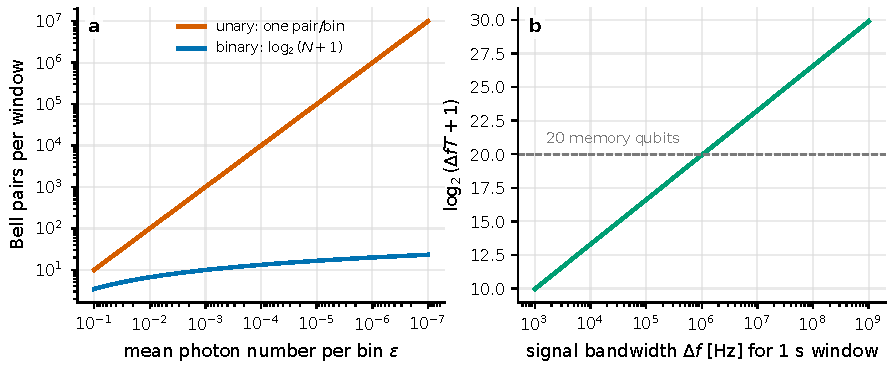
\includegraphics[width=0.94\linewidth]{figures/generated/chapter_17/ch17_timebin_scaling.pdf}
\caption{正是"星光很弱"让时间小格编码有意义。左图比较 unary 与 binary 两种编码对纠缠对的需求：当每格平均光子数 \(\epsilon\) 很小，\(M\sim1/\epsilon\) 个小格可以只用 \(\log_2(M+1)\) 个存储 qubit 来标记。右图显示 \(1\,\mathrm{s}\) 测量窗口里，\(1\,\mathrm{MHz}\) 带宽对应约 \(10^6\) 个小格，也就是约 \(20\) 个 qubit。}
\label{fig:e24-timebin}
\end{figure}

支撑这一切的底层通信技术，是\textbf{量子中继}。为什么不能像放大电信号那样，把量子态放大着往远处传？因为\emph{不可克隆定理}（no-cloning theorem）禁止完美复制一个未知量子态 \citep{1982Natur.299..802W}，而损耗又随距离指数上升（式 \eqref{eq:e24-link-loss}）。中继的思路是分而治之：把长距离切成许多短段，先在每一短段内建立纠缠（短段损耗小、成功率高），再用\textbf{纠缠交换}（entanglement swapping）把相邻短段的纠缠"接龙"成跨越全程的纠缠。理想的中继能把指数损耗换成温和得多的资源缩放，但真实系统还要面对贝尔态测量的成功率、存储寿命、暗计数、门保真度和频率转换等一连串折损。DLCZ 原子系综协议、量子互联网路线以及量子存储综述，都把\emph{存储}放在资源预算的正中央——因为存储的职责，是把这些概率性成功的事件在时间上\emph{对齐}起来 \citep{1998PhRvL..81.5932B,2001Natur.414..413D,2011RvMP...83...33S,2008Natur.453.1023K,2012IEEEN..26d..59V,2006quant.ph..7182U}。

\section{资源账本：纠缠率、存储时间、保真度怎样一起闭合}
\label{sec:e24-budget}

无论上面哪个方案，最后都要回到同一张账本。角分辨率由 \(B\) 白送（式 \eqref{eq:e24-resolution-scale}），可\emph{能不能真的观测}，却要纠缠供应率、存储时间、保真度和星光事件率四项\emph{同时}达标；缺一项，长基线那根相位杠杆就撬不动。

第一项是\textbf{纠缠供应率}。设被接受的有效星光事件率是 \(R_\star\)，每个事件平均消耗 \(n_{\rm pair}\) 个纠缠对，那么

\begin{equation}
  R_{\rm ent}
  \gtrsim
  \frac{n_{\rm pair}\,R_\star}{p_{\rm ready}} .
  \label{eq:e24-entanglement-rate}
\end{equation}
\begin{formulaexplain}
\(R_{\rm ent}\) 是所需的纠缠供应率（单位 Hz），\(R_\star\) 是有效星光事件率（Hz），\(n_{\rm pair}\) 是每个事件消耗的纠缠对数，\(p_{\rm ready}\) 是星光到达时纠缠对已备好的概率。它把天文事件率\emph{直接翻译}成量子网络的吞吐量要求。
\end{formulaexplain}

要读懂这条式子，得先把 \(R_\star\) 讲清楚：它\emph{不是}望远镜收到的总光子率，而是进入了目标空间模式、频率通道、偏振通道、时间窗，并通过质量筛选之后，\emph{真正能用}的事件率。\(p_{\rm ready}\) 越接近 1，说明纠缠资源几乎总是待命，浪费越少。这条式子的启示很直接：对又亮又宽带的源，\(R_\star\) 极高，直接 GJC 会被资源率活活压垮；对又窄带又暗弱的源，\(R_\star\) 小，存储辅助方案才有机会用一个较低的 \(R_{\rm ent}\) 去换取长基线。

第二项是\textbf{存储时间}。最起码，量子态或测量记录要一直存到经典通信和非局域校验都完成为止：

\begin{equation}
  T_{\rm mem}
  \gtrsim
  \max\!\left[\frac{B}{c},\,T_{\rm ent},\,T_{\rm proc},\,T_{\rm win}\right].
  \label{eq:e24-memory-time}
\end{equation}
\begin{formulaexplain}
\(T_{\rm mem}\) 是量子存储必须保持相干的最短时间，等于右边四项取最大：基线光行时 \(B/c\)、纠缠生成时间 \(T_{\rm ent}\)、处理时间 \(T_{\rm proc}\)、测量窗口 \(T_{\rm win}\)。真正卡脖子的往往\emph{不是} \(B/c\)，而是同步和时间小格窗口。
\end{formulaexplain}

代个数字就明白了：光行时 \(B/c=3.3\,\mu\mathrm{s}\times(B/\mathrm{km})\)，所以 \(100\,\mathrm{km}\) 基线只要 \(0.33\,\mathrm{ms}\) 的光行时——听起来很轻松。可 Khabiboulline 型的二进制时间小格方案，为了覆盖窄带弱光，测量窗口 \(T_{\rm win}\) 可能长达 \(\sim1\,\mathrm{s}\)，比光行时严苛好几个数量级。量子存储硬件通常用六个指标来描述：保真度、效率、存储时间、带宽、多模容量、工作波长。对单光子存储，\emph{条件保真度}是读出的波包与写入波包的重合度，\emph{效率}是成功读出光子的概率；一旦要拿存的光子去和星光干涉，这两者的\emph{乘积}、外加相位噪声和模式匹配，都会直接压低最终可见度 \citep{2009NaPho...3..706L,2010EPJD...58....1S,2016JMOp...63.2005H}。

\begin{figure}[tbp]
\centering
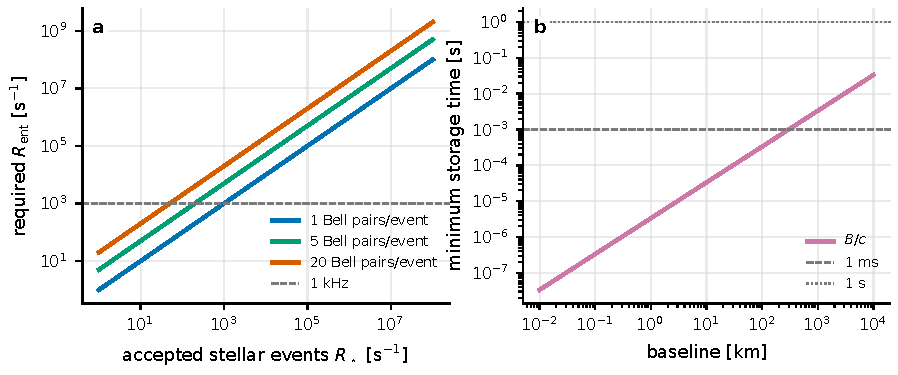
\includegraphics[width=0.94\linewidth]{figures/generated/chapter_17/ch17_entanglement_resources.pdf}
\caption{纠缠率和存储时间给出第一层资源闭合条件。左图把被接受的星光事件率 \(R_\star\) 换成所需纠缠对速率：每个事件消耗的纠缠对越多，需求线抬得越高。右图把基线换成光行时 \(B/c\)：对公里级基线，光行时只是微秒到毫秒，但窄带存储方案常常由测量窗口和纠缠生成时间说了算。}
\label{fig:e24-entanglement-resources}
\end{figure}

第三项是\textbf{保真度}。资源预算里常把链路上几个主要折损因子直接\emph{相乘}，得到一个粗略的有效保真度：

\begin{equation}
  F_{\rm eff}
  \simeq
  F_{\rm Bell}\,
  \eta_{\rm write}\,\eta_{\rm read}\,\eta_{\rm conv}\,
  e^{-T/T_2}\,
  (1-p_{\rm dark})\,
  M_{\rm mode}.
  \label{eq:e24-effective-fidelity}
\end{equation}
\begin{formulaexplain}
\(F_{\rm eff}\) 是粗略的有效资源质量，把纠缠对保真度 \(F_{\rm Bell}\)、写入/读出效率、频率转换效率、存储退相干 \(e^{-T/T_2}\)、暗触发 \((1-p_{\rm dark})\) 与模式匹配 \(M_{\rm mode}\) 全乘在一起。\emph{任何一项偏低，都会乘法式地拉低最终可见度}。
\end{formulaexplain}

逐个点名单位：\(F_{\rm Bell}\)（无量纲，\(\le1\)）是预共享纠缠对的保真度；\(\eta_{\rm write},\eta_{\rm read}\)（无量纲）是写入、读出效率；\(\eta_{\rm conv}\) 是频率转换效率；\(T_2\) 是存储的相干时间（单位 s），\(T\) 是实际存储时长；\(p_{\rm dark}\) 是等效暗触发概率；\(M_{\rm mode}\le1\) 表示频率、时间、偏振、空间四种模式的匹配程度。这不是一条完整的量子信道模型，但它有个好处：\emph{一眼暴露瓶颈}。单看退相干一项，\(T/T_2=1\) 就给 \(e^{-1}\simeq0.37\) 的因子；再假设 \(F_{\rm Bell}=0.8\)、读写各 \(0.7\)、转换 \(0.8\)，暗计数和模式失配还没算，乘起来 \(0.8\times0.7\times0.7\times0.8\simeq0.31\)——最终可见度已经只剩三成上下。这就是为什么这类方案不能只盯着"角分辨率多诱人"，而必须让每一项\emph{同时}闭合。

\begin{figure}[tbp]
\centering
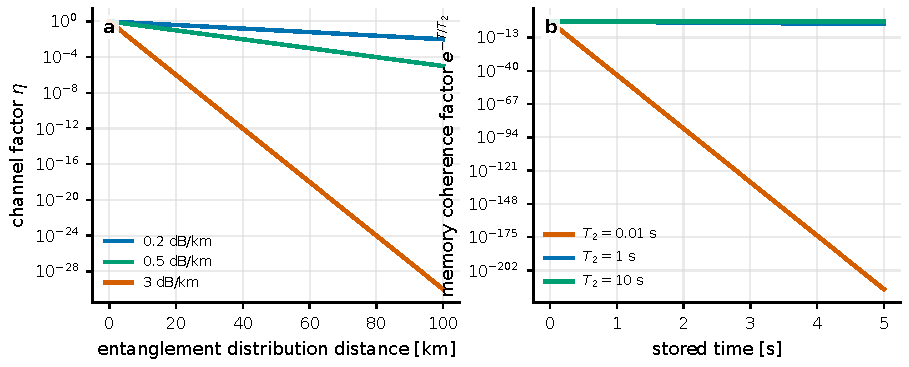
\includegraphics[width=0.94\linewidth]{figures/generated/chapter_17/ch17_fidelity_distance.pdf}
\caption{有效资源质量由链路和存储共同决定。左图给出不同 \(\mathrm{dB\,km^{-1}}\) 损耗下的通道因子随距离的下降；右图给出存储退相干因子 \(e^{-T/T_2}\) 随存储时长的下降。一个长基线方案即使角分辨率再诱人，也要让纠缠对保真度、读写效率、频率转换和存储相干\emph{一起}达标。}
\label{fig:e24-fidelity-distance}
\end{figure}

其中\textbf{频率转换}是天文版本特有的额外难题。许多量子存储材料强耦合的频率并不落在我们想观测的天文波段，而长距离光纤又偏爱电信波段——于是必须做\emph{量子频率转换}：在改变光子频率的同时，保住它的单光子相干、偏振或时间小格编码，还要压住转换过程引入的噪声。尤其要命的是模式匹配：若转换后的谱宽、中心频率、时间波包、偏振和星光对不齐，哪怕只差 \(1\%\)，损失的\emph{也不只是 \(1\%\) 的光子数}——它会直接扣在干涉可见度上，因为可见度衡量的正是两束光"长得有多像" \citep{1990OptL...15.1476K,2010EPJD...58....1S,2016JMOp...63.2005H,2024SPIE13095E..1NR}。

\section{连续变量与辅助单光子：另外两条路各解决什么}
\label{sec:e24-cv-ancilla}

上面的方案都把"左/右路径"当成一个离散的 qubit，再把时间信息塞进存储。还有两类互补的想法，解决的是不同的瓶颈。

第一类是\textbf{连续变量}（continuous variable）路线。这里的"连续变量"指光场的两个正交分量（quadrature），也就是复振幅箭头（第 \ref{chap:e01} 章）的实部和虚部，而不是"左/右"这样非此即彼的离散选择。连续变量的量子隐形传态用一份预共享的\emph{两模压缩真空态}（two-mode squeezed vacuum, TMSV）当资源，靠本地测量把一个模式的正交分量信息转移到远端：

\begin{equation}
  |\psi_{\rm TMSV}\rangle
  =
  \sqrt{1-\lambda^2}\,
  \sum_{n=0}^{\infty}\lambda^n\,|n\rangle_A|n\rangle_B,
  \qquad
  \bar N=2\sinh^2 r .
  \label{eq:e24-tmsv}
\end{equation}
\begin{formulaexplain}
\(|\psi_{\rm TMSV}\rangle\) 是两模压缩真空资源态，\(A,B\) 是相隔很远的两个模式；\(\lambda=\tanh r\)（\(r\) 是压缩参数）控制压缩强度，\(\bar N\) 是总平均光子数。压缩越强，连续变量隐形传态的附加噪声越小，但资源成本越高。
\end{formulaexplain}

这条式子说的是：\(A\) 端和 \(B\) 端的光子数\emph{总是相等}（都取到 \(n\)），而且不同 \(n\) 的振幅按 \(\lambda^n\) 排布——这正是"两模一起被压缩"的量子指纹。理想情形要 \(r\to\infty\)（无穷强压缩）才能无噪声地传送任意连续变量态；现实里 \(r\) 有限，就会掺进一份等效的高斯噪声，通常按 \(e^{-2r}\) 的速度随压缩增强而衰减。Braunstein--Kimble 给出的连续变量隐形传态协议，加上 Gottesman 等的分析，说明这条路能\emph{绕开}离散贝尔测量那个 \(50\%\) 上限；但代价是连续变量的中继更难、远距离的高保真压缩资源也更娇气。最新的最优性分析还提醒：比较不同资源态时，必须把\emph{光子数超选择定则}、局域性和有限的纠缠预算都算进去——压缩度只是账本里的一项，不是全部 \citep{1998PhRvL..80..869B,2012PhRvL.109g0503G,2025PhRvR...7d3278Z}。

第二类是\textbf{辅助单光子}路线，好处是\emph{不依赖长寿命量子存储}。Marchese--Kok 的想法是：让脆弱的星光光子尽早在接收端就地测量掉，改让一个"地面产生、坏了能重做"的辅助单光子去跨基线传输——这样损耗主要落在\emph{可以重来}的地面光子上，而不是不可再生的星光上。对一个小角度的位置估计，相位与角度、以及可达的角度精度满足

\begin{equation}
  \phi=\frac{2\pi B\theta}{\lambda},
  \qquad
  \sigma_\theta
  \ge
  \frac{\lambda}{2\pi B}\,
  \frac{1}{\sqrt{N_{\rm ev}\,\mathcal F_\phi}} .
  \label{eq:e24-angle-fisher}
\end{equation}
\begin{formulaexplain}
左式是角位置 \(\theta\) 与干涉相位 \(\phi\) 的换算；右式是角度误差的下界，\(N_{\rm ev}\) 是有效事件数，\(\mathcal F_\phi\) 是\emph{单个事件}的相位 Fisher 信息（第 \ref{chap:e12} 章）。基线越长、事件越多、单事件信息越高，定位就越精。
\end{formulaexplain}

右式其实就是第 \ref{chap:e12} 章 Fisher 信息 \eqref{eq:e12-fisher-def} 给出的 Cramér--Rao 下界 \eqref{eq:e12-crb} 套在相位估计上的结果：总信息是单事件信息 \(\mathcal F_\phi\) 乘以事件数 \(N_{\rm ev}\)，误差按 \(1/\sqrt{N_{\rm ev}\mathcal F_\phi}\) 下降，前面的 \(\lambda/(2\pi B)\) 是把相位误差换算成角度误差的几何系数——\(B\) 越大，同样的相位误差对应越小的角度误差，这就是长基线的杠杆。Marchese--Kok 在 \(\lambda=628\,\mathrm{nm}\)、光纤衰减长度 \(L_0=10\,\mathrm{km}\) 的模型里，得到十几 \(\mu\mathrm{as}\) 量级的定位标度。Modak--Kok 进一步泼了盆冷水：星光模式占据数 \(\epsilon\ll1\) 和"辅助光子与星光到底有多不可区分"会显著改变收益——若 \(\epsilon\) 从 1 掉到 \(0.01\)，多加辅助光子的好处很快变弱；若模式不可区分度只有 \(96\%\)，三光子方案或许还有赚头，但继续堆更多光子并不一定继续改善 \citep{2023PhRvL.130p0801M,2025PhRvA.111d3701M}。

Padilla、Sajjad、Saif 与 Guha 把问题推到更一般的多模成像极限：先在每个接收站做\emph{本地空间模式排序}（借第 \ref{chap:e12} 章 SPADE 那类技巧），再用预共享纠缠对去模拟一个非局域的合束器乃至更一般的干涉网络。这提醒我们，长基线只是资源的一部分——单孔径内的模式信息、源结构先验、阵列几何、测量基的选择，都会改变最终能榨出的 Fisher 信息。对一对双星的角分离：若只盯着 Rayleigh 标度下的 \(\lambda/B\)，就会错过本地模式排序在\emph{小分离}上的优势；若只追本地超分辨，又拿不到长基线那根相位杠杆。两者要合起来用 \citep{2026PhRvA.113a2608P,2025PhRvR...7d3278Z}。

\section{从实验原型到误差预算}
\label{sec:e24-prototype}

实验原型的价值，不只是证明"能把两个远端节点纠缠起来"，更在于给资源账本里的\emph{每一项都填上可测的数字}。Stas 等在 2026 年的实验，把"非局域相位测量"从线路图搬上了实验台。他们用两个 SiV 金刚石纳米腔节点，配上电子自旋和 \({}^{29}\mathrm{Si}\) 核自旋存储：先生成一对远程纠缠，再让弱信号光在本地与节点相互作用，通过\emph{光子擦除}和非局域的非破坏性预报（heralding）滤掉真空事件。实验里电子贝尔态可达 \(F=0.83(3)\)；纠缠率为 \(13\,\mathrm{Hz}\) 时 \(F\ge0.5\)，降到 \(1.9\,\mathrm{Hz}\) 时 \(F=0.79(3)\)。完整的非局域相位测量中，预报把可见度从"不预报"的 \(0.031(18)\) 提升到 \(0.090(26)\)；再接入 \(1.55\,\mathrm{km}\) 的光纤基线后，核自旋宇称振荡的可见度是 \(0.11(4)\)，而纠缠对保真度仍高于可验证纠缠的阈值，约 \(F=0.63(3)\) \citep{2026Natur.651..326S}。这些数字虽然离天文可用还很远，却第一次把上一节账本里抽象的 \(F_{\rm Bell}\)、\(R_{\rm ent}\)、\(V_{\rm meas}\) 变成了台面上量得出的量。

这类实验的相位误差，由有效试验次数、预报成功率和实测的相位振荡可见度共同决定。用 Fisher 信息写出来：

\begin{equation}
  \mathcal I_\phi
  \simeq
  N_{\rm tr}\,p_{\rm succ}\,V_{\rm meas}^2,
  \qquad
  \mathrm{Var}(\hat\phi)\ge\mathcal I_\phi^{-1} .
  \label{eq:e24-fisher-visibility}
\end{equation}
\begin{formulaexplain}
\(\mathcal I_\phi\) 是总相位 Fisher 信息，\(N_{\rm tr}\) 是试验次数，\(p_{\rm succ}\) 是预报成功概率，\(V_{\rm meas}\) 是实测可见度。可见度以\emph{平方}进入信息量，所以一点点相干损失就会明显放大相位误差；右式是相应的 Cramér--Rao 下界。
\end{formulaexplain}

这里 \(N_{\rm tr}\) 是协议跑了多少次（无量纲），\(p_{\rm succ}\) 是一次试验被接受的概率，\(V_{\rm meas}\) 是相位振荡的可见度。\(V_{\rm meas}^2\) 里的那个平方是关键：可见度掉到 \(1/3\)，信息就掉到 \(1/9\)。而 \(p_{\rm succ}\) 本身又拆成

\begin{equation}
  p_{\rm succ}=\eta_{\rm erasure}\,\eta_{\rm herald}\,P(n_{\rm photon}\ge1),
  \label{eq:e24-psucc}
\end{equation}
\begin{formulaexplain}
\(p_{\rm succ}\) 是一次试验被接受的概率，由光子擦除效率 \(\eta_{\rm erasure}\)、预报探测效率 \(\eta_{\rm herald}\) 和"至少来一个光子"的概率 \(P(n_{\rm photon}\ge1)\) 三者相乘。想提高它，\emph{不能}靠一味加大光强。
\end{formulaexplain}

这条式子藏着一个反直觉的陷阱。你也许会想："成功率 \(p_{\rm succ}\) 越高越好，那就把 \(P(n_{\rm photon}\ge1)\) 拉高——多灌点光子不就行了？"可一旦平均光子数上去，\emph{多光子污染}也跟着上来：一次试验里混进两个甚至更多光子，会破坏干涉、把 \(V_{\rm meas}\) 拉低。而 \(V_{\rm meas}\) 是平方进 \(\mathcal I_\phi\) 的，\(p_{\rm succ}\) 只是一次方——于是 \(p_{\rm succ}\) 涨一点、\(V_{\rm meas}\) 跌一点，总 Fisher 信息 \(\mathcal I_\phi=N_{\rm tr}p_{\rm succ}V_{\rm meas}^2\) 反而\emph{不升反降}。这就是为什么"预报成功率高"不见得是好事。最后把相位误差用式 \eqref{eq:e24-angle-fisher} 换成角度误差：\(B\) 越长，同样的 \(\sigma_\phi\) 对应越小的 \(\sigma_\theta\)，但长基线也会推高纠缠分发的开销、相位锁定的难度和延迟。

\begin{figure}[tbp]
\centering
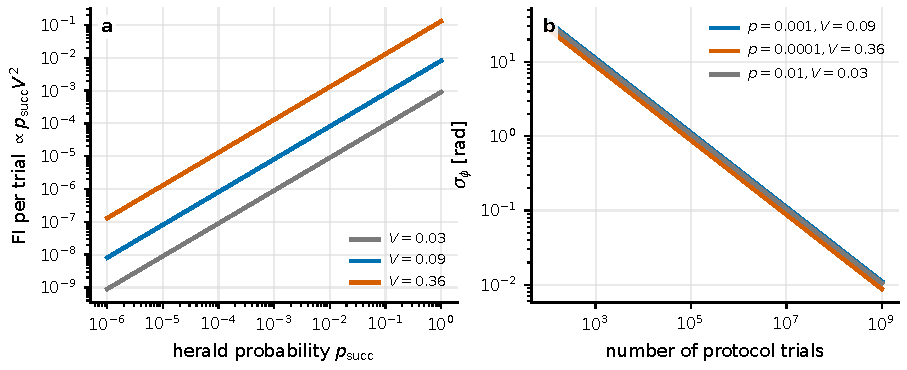
\includegraphics[width=0.94\linewidth]{figures/generated/chapter_17/ch17_fisher_visibility.pdf}
\caption{非局域相位测量的统计收益，同时取决于成功概率和可见度。左图画出单次试验 Fisher 信息的标度 \(p_{\rm succ}V^2\)：可见度降三倍，信息降九倍。右图把试验次数换成相位误差，说明高重复率、低误预报和高纠缠保真度必须\emph{同时}成立，才谈得上有用。}
\label{fig:e24-fisher-visibility}
\end{figure}

Crawford 等的两光子精密天体测量实验，提供了另一级近期台阶：用两个准热光源和时间标记探测器，在桌面模拟装置里看到光子对符合随相位变化的相关行为。这个实验不等于一台完整的量子网络望远镜，但它非常适合当\emph{上天前的排练}——时间标记、偏振匹配、相干时间、HBT 峰拟合、相位稳定、数据筛选，这些环节都和真实的天文弱光观测直接相关 \citep{2023OExpr..3144246C}。

把所有资源摆进同一张图，可以看清我们身处何处：近期实验大致落在 \(R_{\rm ent}\sim1\)–\(10\,\mathrm{Hz}\)、短基线、低有效可见度的角落；而天文可用的"存储辅助窄带"方案，可能需要 \(R_{\rm ent}\sim\mathrm{kHz}\) 到 \(100\,\mathrm{kHz}\)、\(T_{\rm mem}\sim\mathrm{ms}\) 到 \(\mathrm{s}\)、几十个存储 qubit 和很高的模式匹配；宽带成像则更难。四项约束必须\emph{一起}闭合：\(R_{\rm ent}\) 不够会白白浪费星光事件，\(T_{\rm mem}\) 不够会让宇称校验赶不上，\(F_{\rm eff}\) 不够会把可见度洗掉，\(R_\star\) 一旦估错，整套方案可能在第一晚观测之前就已经失去可行性。

\begin{figure}[tbp]
\centering
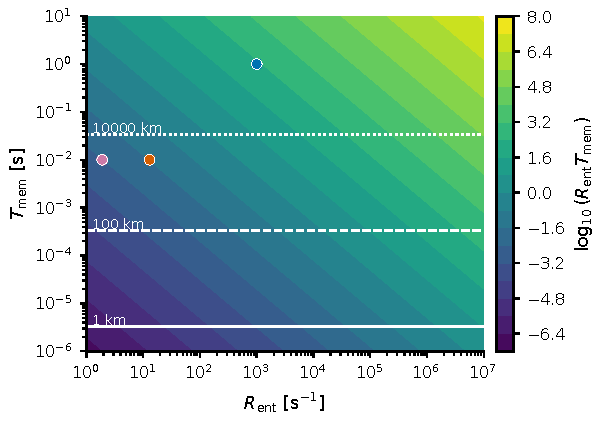
\includegraphics[width=0.94\linewidth]{figures/generated/chapter_17/ch17_network_parameter_space.pdf}
\caption{量子网络望远镜的资源空间，由纠缠率和存储时间共同张开。白线标出 \(1\,\mathrm{km}\)、\(100\,\mathrm{km}\) 和 \(10^4\,\mathrm{km}\) 基线对应的 \(B/c\) 时间；散点给出当前实验的 Hz 级纠缠率与远期 kHz--s 级目标的量级差距。颜色只是资源乘积的标度，完整可行性还要再乘上保真度、模式匹配和天文光子率。}
\label{fig:e24-network-space}
\end{figure}

\section{量子网络和强度干涉怎样互补}
\label{sec:e24-complementarity}

请务必别把量子网络望远镜写成"取代强度干涉"的东西——它是一条\emph{长期互补}的路线。回顾一下两者的分工：第 \ref{chap:e10} 章的强度干涉，靠本地时间标记加离线相关，早就绕开了光学相位传输，几乎不怕大气抖动，代价是主要只拿到 \(|V|^2\)，相位丢了；量子网络路线想\emph{保住}一阶相干的相位，代价则是要支付纠缠、存储、频率转换、预报这一整本资源账。短期内，两者都得和 ELT、VLTI、CHARA、CTAO 以及强度干涉阵列并行发展。

一个务实的分期路线是这样的。\emph{近期}目标是强度干涉和两光子相关：硬件已经接近现成——大面积集光器、SNSPD/SPAD 时间标记、窄带滤光、离线相关，科学目标集中在亮星角直径、双星和发射线区域。\emph{中期}加入本地空间模式排序、两光子天体测量和 GJC 型短基线的上天演示，目标是证明星光模式能和实验室纠缠资源\emph{稳定地干涉}。\emph{远期}才是存储辅助的非局域一阶相干测量，它要求量子存储、频率转换、纠缠分发、纠缠保真度和天文仪器同步一起成熟 \citep{1956Natur.178.1046H,2023OExpr..3144246C,2024SPIE13095E..1NR,2026Natur.651..326S}。

\Needspace{11\baselineskip}
观测规划可以从一个简洁的闭合条件出发：

\begin{equation}
  N_{\rm useful}
  =
  R_\star\,T_{\rm obs}\,
  p_{\rm ready}\,p_{\rm succ}\,V_{\rm meas}^2
  \gtrsim
  N_{\rm req}(\sigma_\theta,\bm{B},\lambda) .
  \label{eq:e24-useful-events}
\end{equation}
\begin{formulaexplain}
\(N_{\rm useful}\) 是真正带相位信息的有效事件数，等于星光事件率、观测时间、资源就绪概率、成功率和可见度平方的乘积；\(N_{\rm req}\) 是达到目标角精度 \(\sigma_\theta\) 所需的事件数。只有 \(N_{\rm useful}\ge N_{\rm req}\)，方案才有观测意义。
\end{formulaexplain}

逐项点名：\(T_{\rm obs}\) 是总观测时间（s），\(N_{\rm req}\) 由目标角精度、阵列几何和模型参数维数决定。这条式子把天文学和量子工程放进了\emph{同一本账}：又亮、又窄带、到达时间或周期已知的信号，会降低资源压力；又暗、又宽带的连续源，则会把所有困难一起放大。值得强调的是，同一本账也适用于更一般的观测设计，只是可观测量从"非局域相位"换成 \(|V|^2\)、\(g^{(2)}\)、偏振角或时间延迟而已。

所以，量子网络望远镜眼下最有价值的产物，\emph{不是}某台已经造好的仪器，而正是这张可以一项项核对的可行性账本。下一章我们回到观测设计的主线：把科学目标落到事件率、通道、基线、背景和协方差上，然后才谈得上在强度干涉、偏振事件表、瞬变触发与未来的非局域相位测量之间做取舍。

\section*{本章要点}
\addcontentsline{toc}{section}{本章要点}

\begin{itemize}
\item \textbf{瓶颈的来源。} 长基线振幅干涉要把稀少的星光单光子送到同一个合束器，可链路损耗随距离\emph{指数}上升（式 \eqref{eq:e24-link-loss}），而基线越长分辨率越高（式 \eqref{eq:e24-resolution-scale}）——诱惑和困难来自同一个量纲。
\item \textbf{换掉要搬运的东西。} Gottesman--Jennewein--Croke 用一个已知、可验证、可重来的预共享纠缠光子 \eqref{eq:e24-lab-entangled-photon} 替代长途搬运星光；扫描本地相位 \(\delta\) 就能从符合点击率 \eqref{eq:e24-gjc-probability} 读出复可见度 \(V\)。线性光学的贝尔测量带来约 \(50\%\) 的事件损失。
\item \textbf{弱光的稀疏性是朋友。} 每个窗口平均只有 \(\epsilon\ll1\) 个星光光子，于是二进制时间小格编码把资源从 \(M\sim1/\epsilon\) 个纠缠对压到约 \(\log_2 M\) 个存储 qubit（式 \eqref{eq:e24-binary-timebin}）——量子中继与量子存储负责把概率性成功事件对齐。
\item \textbf{四项要一起闭合。} 纠缠供应率 \eqref{eq:e24-entanglement-rate}、存储时间 \eqref{eq:e24-memory-time}、有效保真度 \eqref{eq:e24-effective-fidelity} 和有效星光事件率必须同时达标；保真度是各因子\emph{相乘}，任一项偏低都会乘法式洗掉可见度。频率转换的模式失配尤其致命。
\item \textbf{还有两条互补路。} 连续变量隐形传态用两模压缩真空 \eqref{eq:e24-tmsv} 绕开 \(50\%\) 上限但资源更娇气；辅助单光子路线 \eqref{eq:e24-angle-fisher} 让可重来的地面光子去承担链路风险，收益却对 \(\epsilon\) 和模式不可区分度敏感。
\item \textbf{可见度以平方进信息。} 实验的相位 Fisher 信息标度为 \(p_{\rm succ}V_{\rm meas}^2\)（式 \eqref{eq:e24-fisher-visibility}）；一味加大光强会引入多光子污染、压低 \(V_{\rm meas}\)，反而降低总信息——量子网络与强度干涉应当分期并行、长期互补（式 \eqref{eq:e24-useful-events}）。
\end{itemize}

\medskip
\noindent\textbf{想一想。}
\begin{enumerate}
\item 若把观测带宽 \(\Delta\nu\) 从 \(10\,\mathrm{GHz}\) 收窄到 \(1\,\mathrm{MHz}\)，直接 GJC 路线每秒要准备的纠缠光子数、以及二进制时间小格方案所需的存储 qubit 数，各会怎样变化？为什么"窄带"反而对存储辅助方案有利？
\item 在有效保真度 \eqref{eq:e24-effective-fidelity} 里，若你只能改善一个环节，你会先攻哪一项？把 \(T/T_2\)、读写效率、频率转换效率各改善 \(10\%\)，分别对 \(F_{\rm eff}\) 带来多大提升？
\item 为什么"提高预报成功率 \(p_{\rm succ}\)"不一定提高总 Fisher 信息 \(\mathcal I_\phi\)？用式 \eqref{eq:e24-fisher-visibility} 和 \eqref{eq:e24-psucc} 说明多光子污染在什么条件下会让收益反转。
\end{enumerate}
